\documentclass[11pt,a4paper]{article}
\usepackage[lmargin=1.0in,rmargin=1.0in,bottom=1.0in,top=1.0in,twoside=False]{geometry}

\usepackage{inconsolata}
\usepackage{libertine}

\usepackage{amssymb,amsmath,amsthm}
\usepackage{mathtools}
\usepackage{graphicx}\usepackage{enumerate}
\usepackage{tikz}
\usetikzlibrary{shapes}

\usepackage[T1]{fontenc}

\usepackage{enumitem}

\usepackage{microtype}
\usepackage{amsfonts}
\usepackage{comment}
\usepackage{mathrsfs}
\setlength{\marginparwidth}{2cm}
\usepackage{todonotes}
\newcommand{\mpil}[2][]{\todo[color=magenta!80,#1]{{\textbf{MaPi:} #2}}}
\newcommand{\mipil}[2][]{\todo[color=orange!30,#1]{\small {\textbf{MiPi:} #2}}}
\newcommand{\gs}[2][]{\todo[color=blue!20,#1]{\small {\textbf{GS:} #2}}}
\newcommand{\kk}[2][]{\todo[color=green!20,#1]{\small {\textbf{KK:} #2}}}

\definecolor{blue}{rgb}{0.1,0.2,0.5}
\definecolor{brown}{rgb}{0.6,0.6,0.2}
\usepackage[ocgcolorlinks, linkcolor={blue}, citecolor={brown}]{hyperref}
\usepackage{cleveref}

\usepackage{enumerate}
\usepackage{latexsym}

\usepackage{soul}

\newtheorem{lemma}{Lemma}[section]
\newtheorem{observation}{Observation}[section]
\newtheorem{claim}{Claim}[section]
\newtheorem{theorem}[lemma]{Theorem}
\newtheorem{corollary}[lemma]{Corollary}
\newtheorem{conjecture}[lemma]{Conjecture}

\newcommand{\Oh}{\mathcal{O}}

\newcommand{\argmax}{\text{argmax}}
\newcommand{\argmin}{\text{argmin}}

\newcommand{\distprofile}[3]{\mathrm{prof}_{#1,#2}[#3]}
\newcommand{\tildeprofile}[3]{\widetilde{\mathrm{prof}}_{#1,#2}[#3]}
\newcommand{\barprofile}[3]{\overline{\mathrm{prof}}_{#1,#2}[#3]}

\newcommand{\hatprofile}[3]{\widehat{\mathrm{prof}}_{#1,#2}[#3]}
\newcommand{\diststarprofile}[3]{\mathrm{prof}^\star_{#1,#2}[#3]}
\newcommand{\dist}{\mathrm{dist}}
\newcommand{\ecc}{\mathrm{ecc}}

\renewcommand{\leq}{\leqslant}
\renewcommand{\geq}{\geqslant}
\renewcommand{\le}{\leqslant}
\renewcommand{\ge}{\geqslant}
\renewcommand{\setminus}{-}

\usepackage{marvosym}

\newcommand{\cutgraph}{\textrm{\CutLeft}}

\usepackage{textpos}


\begin{document}

\author{
  Kacper Kluk\thanks{Institute of Informatics, University of Warsaw, Poland. \texttt{k.kluk@uw.edu.pl}}
  \and
  Marcin Pilipczuk\thanks{Institute of Informatics, University of Warsaw, Poland. \texttt{m.pilipczuk@uw.edu.pl}}
  \and
  Micha\l{} Pilipczuk\thanks{Institute of Informatics, University of Warsaw, Poland. \texttt{michal.pilipczuk@mimuw.edu.pl}}
  \and
  Giannos Stamoulis\thanks{IRIF, Université Paris Cité, CNRS, Paris, France. \texttt{giannos.stamoulis@irif.fr}}
}


\title{Faster diameter computation in graphs of bounded Euler genus\thanks{
  K.K. and Ma.P. are supported by Polish National Science Centre SONATA BIS-12 grant number 2022/46/E/ST6/00143.
  This work is a part of project BOBR (Mi.P., G.S.) that has received funding from the European Research Council (ERC) 
under the European Union's Horizon 2020 research and innovation programme (grant agreement No.~948057). In particular, a majority of work on this manuscript was done while G.S. was affiliated with University of Warsaw.}}

\date{}

\maketitle

\begin{abstract}
We show that for any fixed integer $k \geq 0$, there exists an algorithm
that computes the diameter and the eccentricies of all vertices of an input
unweighted, undirected $n$-vertex graph of Euler genus at most $k$ in time
 \[ \Oh_k(n^{2-\frac{1}{25}}). \]
Furthermore, for the more general class of graphs
that can be constructed
by clique-sums from graphs that are of Euler genus at most $k$ after deletion
of at most $k$ vertices, we show an algorithm for the same task that achieves the running time bound
 \[ \Oh_k(n^{2-\frac{1}{356}} \log^{6k} n). \]
Up to today, the only known subquadratic algorithms for computing the diameter in those graph classes
are that of [Ducoffe, Habib, Viennot; SICOMP 2022], [Le, Wulff-Nilsen; SODA 2024],
and [Duraj, Konieczny, Pot\k{e}pa; ESA 2024]. These algorithms work
in the more general setting of $K_h$-minor-free graphs,
but the running time bound is $\Oh_h(n^{2-c_h})$ for some constant $c_h > 0$ depending
on $h$. 
That is, our savings in the exponent, as compared to the naive quadratic algorithm, 
are independent of the parameter $k$.

The main technical ingredient of our work is an improved bound on the number of distance
profiles, as defined in [Le, Wulff-Nilsen; SODA 2024], in graphs of bounded Euler genus.
\end{abstract}


\begin{textblock}{20}(11.8,4.35)
  \includegraphics[width=60px]{ERC2.jpg}
\end{textblock}


\section{Introduction}

Computing the diameter of an input (undirected, unweighted) graph $G$ is a classic computational 
problem that can be trivially solved in $\Oh(nm)$ time\footnote{We follow the convention that the vertex and the edge count of the input graph are denoted by $n$ and $m$, respectively.}.
In 2013, Roditty and Vassilevska-Williams showed that this running
time bound cannot be significantly improved in general:
any algorithm distinguishing graphs of diameter $2$ and $3$
running in time $\Oh(m^{2-\varepsilon})$, for any fixed $\varepsilon > 0$,
would break the Strong Exponential Time Hypothesis~\cite{RodittyW13}. 
This motivates the search for restrictions on $G$ that would make the  problem of computing the diameter more tractable.

As shown by Cabello and Knauer~\cite{CabelloK09}, sophisticated orthogonal range query data structures allow near-linear diameter
computation in graphs of constant treewidth.
A breakthrough result by Cabello~\cite{Cabello19} showed that 
the diameter of an $n$-vertex planar graph can be computed in $\widetilde{\Oh}(n^{11/6})$ time;
this complexity has been later improved by Gawrychowski, Kaplan, Mozes, Sharir, and Weimann to
$\widetilde{\Oh}(n^{5/3})$~\cite{GawrychowskiKMS21}\footnote{The $\widetilde{\Oh}(\cdot)$ notation hides factors polylogarithmic in $n$, and the $\Oh_k(\cdot)$ notation hides factors depending on a parameter $k$.}.
A subsequent line of research~\cite{DucoffeHV22,DurajKP23,LeW24}
generalized this result to $K_h$-minor-free graphs:
for every integer $h$, there exists a constant $c_h > 0$ such that the diameter
problem in $n$-vertex $K_h$-minor-free graphs can be solved in time $\Oh_h(n^{2-c_h})$. 
In the works~\cite{DurajKP23,LeW24}, it holds that $c_h = \Omega\left(\frac{1}{h}\right)$; so the savings tend to zero as the size of the excluded clique minor increases.

However, known lower bounds, including the one of~\cite{RodittyW13}, does not exclude the possibility
that $c_h$ can be made a universal constant. That is, no known lower bound refutes
the following conjecture:
\begin{conjecture}\label{conj:taunt}
There exists a constant $c > 0$ such that,
for every integer $h > 1$, the diameter problem in (unweighted, undirected) $n$-vertex
$K_h$-minor-free graphs can be solved in time $\Oh_h(n^{2-c})$. 
\end{conjecture}

\paragraph{Graphs of bounded Euler genus.}
Our main result is the verification of \Cref{conj:taunt} for graphs
of bounded Euler genus. Furthermore, our algorithm computes also the eccentricies
of all the vertices of the input graph $G$. Recall here that
    the eccentricity of a vertex $v \in V(G)$ is defined as
    $\ecc(v) \coloneqq \max_{u \in V(G)} \dist_G(u,v)$, where $\dist_G(\cdot,\cdot)$ is the distance metric in $G$.
\begin{theorem}\label{thm:main-genus}
For every integers $k \geq 1$,
there exists an algorithm that, given an (unweighted, undirected) $n$-vertex graph $G$
of Euler genus at most $k$, runs in time $\Oh_k(n^{2-\frac{1}{25}})$
and computes the diameter of $G$ and the eccentricity of every vertex of $G$.
\end{theorem}

We remark that in~\cite[Section~9]{Cabello19}, Cabello briefly speculated that his approach could be also generalized to graphs embeddable on surfaces of bounded genus. However, as noted in \cite{Cabello19}, this would require significant effort, as the technique works closely on the embedding and in surfaces of higher genus, additional topological hurdles arise. In contrast, in our proof of \Cref{thm:main-genus} the main ingredient is an improved combinatorial bound on the number of so-called \emph{distance profiles}~\cite{LeW24} in graphs of bounded Euler genus. This proof uses topology only very lightly, while the rest of the argument is rather standard and topology-free. All in all, we obtain a robust methodology of approaching the problem, which, as we will see, can be also used to attack \Cref{conj:taunt} to some extent.

To explain our bound on distance profiles, we need to recall several relevant definitions.

Let $G$ be a graph, $R \subseteq V(G)$ be a subset of vertices, and $s_R \in R$ be a vertex in $R$.
The \emph{distance profile} of a vertex $u \in V(G)$ to $R$ (relative to $s_R$)
  is the function $\distprofile{R}{s_R}{u} \colon R \to \mathbb{Z}$ defined as follows:
  \[ \distprofile{R}{s_R}{u}(s) = \dist_G(u,s) - \dist_G(u,s_R)\qquad \textrm{for all }s\in R. \]
Note that provided $R$ is connected\footnote{A subset of vertices $R$ of a graph $G$ is {\em{connected}} if the induced subgraph $G[R]$ is connected.}, we have
$\distprofile{R}{s_R}{u}(s) \in \{-|R|,-|R|+1,\ldots,|R|-1,|R|\}$. In~\cite{LeW24},
Le and Wulff-Nilsen proved that if $R$ is connected and $G$ is $K_h$-minor-free, then
the set system $$\left\{ \left\{(s,i) \in R \times \{-|R|,\ldots,|R|\}~|~i \leq \distprofile{R}{s_R}{u}(s)\right\}~\colon~u \in V(G)\right\}$$ has VC dimension at most $h-1$. Hence, by applying the Sauer-Shelah Lemma we obtain that
\begin{theorem}[\cite{LeW24}]\label{thm:distprofiles-LeW24}
For every integer $h\geq 1$, $K_h$-minor-free graph $G$, connected set $R \subseteq V(G)$, and  $s_R \in R$, there are at most $\Oh_h(|R|^{2h-2})$
different distance profiles to $R$ relative to $s_R$. 
\end{theorem}
The VC dimension argument applied above inevitably leads to a bound with the exponent depending on $h$.
We show that for  graphs of bounded Euler genus, the bound of \Cref{thm:distprofiles-LeW24}
can be improved to a polynomial of degree independent of the parameter.
\begin{theorem}\label{thm:distprofiles}
For every integer $k\geq 1$, (unweighted, undirected) graph $G$ of Euler genus at most~$k$, connected set $R \subseteq V(G)$, and $s_R \in R$,
the number of distance profiles to $R$ relative to $s_R$
is at most~$\Oh_k(|R|^{12})$.
\end{theorem}
The main idea behind the proof of \Cref{thm:distprofiles} is the following simple
observation:
if $P$ is a shortest path from some $u \in V(G)$ to $s_R$, then, as one walks along $P$
from $u$ to $s_R$, the distance profile of the current vertex to $R$ can only (point-wise) increase.
A slightly more technical modification of this argument works for shortest paths
from $u \in V(G)$ to $R$. This allows us to reduce the case of bounded Euler genus graphs
to the planar case by cutting along a constant number of shortest-to-$R$ paths,
and analysing how the distance profiles change during such a process.

One could ask whether an improvement similar to that of \Cref{thm:distprofiles}
would be possible even in the generality of $K_h$-minor-free graphs.
Unfortunately, it seems that \Cref{thm:distprofiles} is the limit of such improvements. More precisely, the following simple example shows that the linear dependency on $h$ in the exponent of the bound on the number of profiles is inevitable even in graphs of treewidth $h$ (which are  $K_{(h+1)^2}$-minor-free).


Let $0 < k \ll \ell$ be positive integers.
Let $R$ be a path of length $\ell$ and $v_1,\ldots,v_k$ be $k$ equidistant
points on $R$ (i.e., the distance between $v_i$ and $v_{i+1}$ is at least $p \coloneqq \lfloor \ell/(k-1) \rfloor$).
For every vector $\mathbf{a} = (a_1,\ldots,a_k) \in \{\ell, \ldots, \ell + p \}^k$,
construct a vertex $u(\mathbf{a})$ and, for every $i\in \{1,\ldots,k\}$, connect it with
$v_i$ using a path of length $a_i$.
This finishes the construction of the graph $G$; see~\Cref{fig:example} for an illustration.
Note that $G$ has treewidth at most $k+1$, because $G-\{v_1,\ldots,v_k\}$ is a forest.
Furthermore, since the distance between consecutive vertices $v_i$ is at least $p$, we have that
  $\dist_G(u(\mathbf{a}), v_i) = a_i$ for every vector $\mathbf{a}$ and $i\in \{1,\ldots,k\}$.
Consequently, if we restrict to vectors $\mathbf{a}$ with $a_1 = \ell$, 
every vertex $u(\mathbf{a})$ has a different distance profile to $R$ relative to $v_1$.
Finally, note that there are $(p + 1)^{k-1} \geq (\ell/(k-1))^{k-1} = \Omega_k(\ell^k)$ different
vectors $\mathbf{a}$ with $a_1=\ell$, giving that many different~profiles.
\begin{figure}[ht]
  \centering
  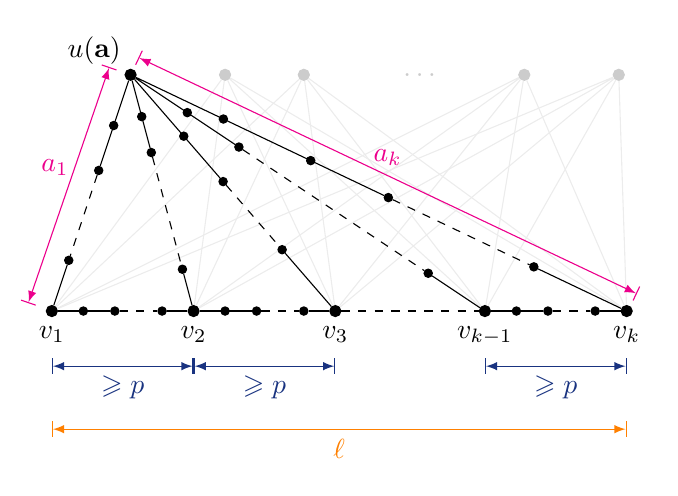
\begin{tikzpicture}
    \tikzset{black node/.style={draw, circle, fill = black, minimum size = 4pt, inner sep = 0pt}}
    \tikzset{small black node/.style={draw, circle, fill = black, minimum size = 3pt, inner sep = 0pt}}

    \node[black node, label={below:$v_1$}] (A) at (0,0) {};
    \node[black node, label={below:$v_2$}] (B) at (1.8,0) {};
    \node[black node, label={below:$v_3$}] (C) at (3.6,0) {};
    \node[black node, label={below:$v_{k-1}$}] (D) at (5.5,0) {};
    \node[black node, label={below:$v_k$}] (E) at (7.3,0) {};

  
    \node[small black node] at (0.4,0) {};
    \node[small black node] (Al) at (0.8,0) {};
    \node[small black node] (Ar) at (1.4,0) {};

    \node[small black node] at (2.2,0) {};
    \node[small black node] (Bl) at (2.6,0) {};
    \node[small black node] (Br) at (3.2,0) {};

    \node[small black node] at (5.9,0) {};
    \node[small black node] (Dl) at (6.3,0) {};
    \node[small black node] (Dr) at (6.9,0) {};


    \draw (A) -- (Al) (Ar) -- (B)
          (B) -- (Bl) (Br) -- (C)      
          (D) -- (Dl) (Dr) -- (E);
    \draw[dashed] (Al) -- (Ar) (Bl) --  (Br) (C) -- (D) (Dl) -- (Dr);

    \draw[blue] (0,-7mm) coordinate (S) edge[|<->|, >= latex] node[below]{\textcolor{blue}{$\ge p$}} (1.8,-7mm);
    \draw[blue] (1.8,-7mm) coordinate (S) edge[|<->|, >= latex] node[below]{\textcolor{blue}{$\ge p$}} (3.6,-7mm);
    \draw[blue] (5.5,-7mm) coordinate (S) edge[|<->|, >= latex] node[below]{\textcolor{blue}{$\ge p$}} (7.3,-7mm);
    \draw[orange] (0,-15mm) coordinate (S) edge[|<->|, >= latex] node[below]{\textcolor{orange}{$\ell$}} (7.3,-15mm);

    \node[black node, label={[label distance=-2pt]120:$u(\mathbf{a})$}] (X) at (1,3) {};
    
    \node[black node,gray!40!white] (T) at (2.2,3) {};
    \node[black node,gray!40!white] (P) at (3.2,3) {};
    \node[black node,gray!40!white] (Q) at (6,3) {};
    \node[black node,gray!40!white] (R) at (7.2,3) {};
    \node[label={center:\textcolor{gray!40!white}{$\dots$}}] at (4.7,3) {};
    \draw[gray!15!white] (T) -- (A) (T) -- (B) (T) -- (C) (T) -- (D) (T) -- (E);
    \draw[gray!15!white] (P) -- (A) (P) -- (B) (P) -- (C) (P) -- (D) (P) -- (E);
    \draw[gray!15!white] (Q) -- (A) (Q) -- (B) (Q) -- (C) (Q) -- (D) (Q) -- (E);
    \draw[gray!15!white] (R) -- (A) (R) -- (B) (R) -- (C) (R) -- (D) (R) -- (E);

    \path (X) to node[small black node] [pos=0.2] {}  node[small black node] [pos=0.4] (X1) {} 
    node[small black node] [pos=0.8] (X2) {}(A);
    \path (X) to node[small black node] [pos=0.16] {}  node[small black node] [pos=0.32] (Y1) {} 
    node[small black node] [pos=0.84] (Y2) {}(B);
    \path (X) to node[small black node] [pos=0.25] {}  node[small black node] [pos=0.45] (Z1) {} 
    node[small black node] [pos=0.75] (Z2) {}(C);
    \path (X) to node[small black node] [pos=0.15] {}  node[small black node] [pos=0.3] (W1) {} 
    node[small black node] [pos=0.85] (W2) {}(D);
    \path (X) to node[small black node] [pos=0.18] {} node[small black node] [pos=0.36] {}  node[small black node] [pos=0.52] (V1) {} 
    node[small black node] [pos=0.82] (V2) {}(E);

    \draw (X) -- (X1) (X2) -- (A)
    (X) -- (Y1) (Y2) -- (B)
    (X) -- (Z1) (Z2) -- (C)
    (X) -- (W1) (W2) -- (D)
    (X) -- (V1) (V2) -- (E);
    \draw[dashed] (X1) -- (X2)  (Y1) -- (Y2) (Z1) -- (Z2) (W1) -- (W2) (V1) -- (V2);

    \draw[magenta] (0.73,3.1) coordinate edge[|<->|, >= latex] node[above]{\textcolor{magenta}{$a_1$~~~}} (-0.3,0.1);
    \draw[magenta] (1.1,3.22) coordinate edge[|<->|, >= latex] node[above]{\textcolor{magenta}{$a_k$}} (7.43,0.22);


  \end{tikzpicture}
  \caption{Illustration of a construction that shows that linear dependency on $h$ in the exponent of the bound on the number of profiles is inevitable, even in graphs of treewidth $h$.}
  \label{fig:example}
\end{figure}

Our algorithm for \Cref{thm:main-genus} follows closely the approach of Le and Wulff-Nilsen~\cite{LeW24} augmented by the bound provided by \Cref{thm:distprofiles}. Namely, we first compute an $r$-division of the input graph $G$
into regions of size $r=n^{\delta}$, for some small $\delta > 0$. Then we use \Cref{thm:distprofiles}
for individual regions $R$ to speed up the computation of distances between $R$ and $V(G) \setminus R$,
by grouping vertices outside $R$ according to their distance profiles 
to $R$. Each group is batch-processed in a single step.


\paragraph{Generalizations.}
Further, we show that our techniques combine well with the techniques for bounded
treewidth graphs of Cabello and Knauer~\cite{CabelloK09}.
First, we show that \Cref{conj:taunt} holds for classes of graphs
of bounded Euler genus with a constant number of \emph{apices}, i.e., vertices that are arbitrarily connected to the rest of the graph.

\begin{theorem}\label{thm:main-apices}
For every integers $g,k \geq 1$, 
there exists an algorithm that, given an (unweighted, undirected) $n$-vertex graph $G$
and a set $A \subseteq V(G)$ such that $|A| \leq k$ and $G-A$ is
of Euler genus at most $g$, runs in time $\Oh_{g,k}(n^{2-\frac{1}{25}} \log^{k-1} n)$
and computes the diameter of $G$ and the eccentricity of every vertex of $G$.
\end{theorem}
Second, we show that \Cref{conj:taunt} holds for classes of graphs
constructed by clique-sums of graphs as in \Cref{thm:main-apices}.
To state this result formally, we need some definitions. For a graph $G$,
   a \emph{tree decompostion} of $G$ is a pair $(T,\beta)$ where $T$ is a tree
  and $\beta$ is a function that assigns to every $t \in V(T)$ a \emph{bag} 
  $\beta(t) \subseteq V(G)$ such that (1) for every $v \in V(G)$, the set $\{t \in V(T)~|~v \in \beta(t)\}$ is nonempty and connected in $T$, and (2) for every $uv \in E(G)$ there exists $t \in V(T)$ with $u,v \in \beta(t)$. 
 The \emph{torso} of the bag $\beta(t)$ is constructed from $G[\beta(t)]$ by adding, for every
 neighbor $s$ of $t$ in $T$, all edges between the vertices of $\beta(s) \cap \beta(t)$.
\begin{theorem}\label{thm:main-decomp}
For every integer $k \geq 1$, 
there exists an algorithm with the following specification.
The input consists of an (unweighted, undirected) $n$-vertex graph $G$
together with a tree decomposition $(T,\beta)$ of $G$ and a set $A(t) \subseteq \beta(t)$ for
every $t \in V(T)$ satisfying the following properties:
\begin{itemize}[nosep]
\item For every node $t \in V(T)$, we have that $|A(t)| \leq k$ and the torso of $\beta(t)$ with the vertices
of $A(t)$ deleted is a graph of Euler genus at most $k$.
\item For every edge $st \in E(T)$, we have $|\beta(s) \cap \beta(t)| \leq k$.
\end{itemize}
The algorithm runs in time $\Oh_k(n^{2-\frac{1}{356}} \log^{6k} n)$ and computes
the diameter of $G$ and the eccentricity of every vertex of $G$.
\end{theorem}
Note that the statements of
\Cref{thm:main-apices,thm:main-decomp} require the set $A$ and
the decomposition $(T,\beta)$, respectively, to be provided explicitly on input;
this should be compared with more general statements where the algorithm is 
given only $G$ with a promise that such set $A$ or decomposition $(T,\beta)$ exist. At this point, we are not aware of any existing algorithm that would find in subquadratic time a set $A$ as in \Cref{thm:main-apices},
or the decomposition $(T,\beta)$ with the sets $A$ as in \Cref{thm:main-decomp}, even in the approximate sense. However, we were informed by Korhonen, Pilipczuk, Stamoulis, and Thilikos~\cite{KorhonenPST24priv} that it seems likely that the techniques introduced in the recent almost linear-time algorithm for minor-testing~\cite{KorhonenPS24} could be used to construct such an algorithm, with almost linear time complexity. With this result in place, the assumption about the decomposition and/or apex sets being provided on input could be lifted in \Cref{thm:main-apices,thm:main-decomp}; this is, however, left to future work.


\paragraph{Discussion.}
As one of the main outcomes of their theory of graph minors, Robertson and Seymour proved the following Structure Theorem~\cite{RobertsonS03a}: every $K_h$-minor-free graph $G$
admits a tree decomposition $(T,\beta)$ such that
\begin{itemize}[nosep]
 \item for every pair $s,t$ of adjacent nodes of $T$, the set $\beta(t) \cap \beta(s)$ has size $\Oh_h(1)$; and
 \item the torso of every bag $\beta(t)$ is ``nearly embedable'' into a surface of bounded (in terms of $h$) Euler~genus.
\end{itemize}
The notion of being ``nearly embeddable'' encompasses adding a constant number of apices (which can be handled by \Cref{thm:main-decomp}) and a constant number of so-called
vortices (which are not handled by \Cref{thm:main-decomp}). Thus, our methods fall short of verifying  \Cref{conj:taunt} in full generality due to vortices.

We remark that recently, Thilikos and Wiederrecht~\cite{ThilikosW22} proved a variant of the Structure Theorem, where under the stronger assumption of excluding a minor of a {\em{shallow vortex grid}}, instead of a clique minor, they gave a decomposition as above, but with torsos devoid of vortices. Thus, the decomposition for shallow-vortex-grid-minor-free graphs provided by~\cite{ThilikosW22} can be directly plugged into \Cref{thm:main-decomp}, with the caveat that~\cite{ThilikosW22} does not provide a subquadratic algorithm to compute the decomposition.

Coming back to \Cref{conj:taunt},
the simplest case
that we are currently unable to solve is the setting when the input is a planar graph plus a single vortex. More formally, for a fixed integer $k$, let $\mathcal{G}_k$ be the class of graphs
defined as follows. We have $G \in \mathcal{G}_k$ if there exist two subgraphs $G_0,G_1$
of $G$ and a sequence of vertices $v_1,\ldots,v_b$ in $V(G_0) \cap V(G_1)$
such that:
\begin{itemize}[nosep]
 \item $V(G) = V(G_0) \cup V(G_1)$,
 \item $E(G) = E(G_0) \cup E(G_1)$,
 \item $G_0$ admits a planar embedding where the vertices $v_1,\ldots,v_b$ lie on one face in
this order, and
\item $G_1$ admits a tree decomposition $(T_1,\beta_1)$, where $T_1$ is a path on nodes $t_1,\ldots,t_b$ and for every $i\in\{1,\ldots,b\}$, the bag $\beta_1(t_i)$ contains $v_i$
and is of size at most $k$.
\end{itemize}
It is easy to see that graphs from $\mathcal{G}_k$ are $K_{k+\Oh(1)}$-minor-free.
Do they satisfy \Cref{conj:taunt}? That is, is there a constant
$c > 0$ such that the diameter problem in $\mathcal{G}_k$ can be solved in
time $\Oh_k(n^{2-c})$?

\paragraph{Organization.}
We prove \Cref{thm:distprofiles} in \Cref{sec:distprofiles}.
\Cref{thm:main-apices} is proven in \Cref{sec:algo-genus}; note that \Cref{thm:main-genus} follows from \Cref{thm:main-apices}
for $k=1$. 
\Cref{thm:main-decomp} is proven in \Cref{sec:algo}.

 
\section{Preliminaries}\label{sec:prelims}

\paragraph{Set systems and VC-dimension.}
A \emph{set system} is a collection $\mathcal{F}$ of subsets of a given set $A$, which we call \emph{ground set} of $\mathcal{F}$.
We say that a subset $Y\subseteq A$ is \emph{shattered by} $\mathcal{F}$
if $\{Y \cap S : S \in \mathcal{F}\} = 2^Y$, that is, the intersections of $Y$ and the sets in $\mathcal{F}$ contain every subset of $Y$.
The \emph{VC-dimension} of a set system $\mathcal{F}$ with ground set $A$
is the size of the largest subset $Y\subseteq A$ shattered by $\mathcal{F}$. The notion of VC-dimension was introduced by Vapnik and Chervonenkis~\cite{VapnikC71}.

We will use the following well-known Sauer-Shelah Lemma~\cite{Sauer72,Shelah72}, which gives a polynomial upper bound on the size of a set system of bounded VC-dimension.

\begin{lemma}[Sauer-Shelah Lemma]\label{lem:sauer-shelah}
  Let $\mathcal{F}$ be a set system with ground set $A$.
  If the VC-dimension of $\mathcal{F}$ is at most $k$, then $|\mathcal{F}|=\mathcal{O}(|A|^k)$.
\end{lemma}

\paragraph{Basic graph notation.} All our graphs are undirected.
For a graph $G$, the neighborhood of a vertex $u$ is defined as $N_G(u) = \{v~\colon~uv \in E(G)\}$
and for $X \subseteq V(G)$ we have $N_G(X) = \bigcup_{u \in X} N_G(u) \setminus X$. 

The {\em{length}} of a path $P$, denoted $|P|$, is the number of edges of $P$.
For two vertices $u,v$ of a graph $G$, the {\em{distance}} between $u$ and $v$,
denoted $\dist_G(u,v)$, is defined as the minimum length of a path in $G$ with endpoints $u$ and $v$.
For every $v\in V(G)$ and set $R \subseteq V(G)$, we set $\dist_G(v,R)\coloneqq \min\{\dist_G(v,y)\colon y\in R\}.$
For vertices $x,y$ appearing on a path $P$, by $P[x,y]$ we denote the subpath of $P$ with endpoints $x$ and $y$.
The set of vertices traversed by a path $P$ is denoted by $V(P)$.
In all above notation, we sometimes drop the subscript if the graph is clear from the context.

For a nonnegative integer $q$, we use the shorthand $[q]\coloneqq\{1,\ldots,q\}$.
For a vertex $v \in V(G)$ and a set $X \subseteq V(G)$, we define the \emph{$X$-eccentricity} of $v$ as
$\ecc_X(v) \coloneqq \max_{x \in X} \dist(v,x)$.
Thus, the eccentricity of $v$ in $G$ is the same as its $V(G)$-eccentricity.

The \emph{Euler genus} of a graph $G$ is the minimum Euler characteristic of a surface, where $G$ is embeddable.
We refer to the textbook of Mohar and Thomassen for more on surfaces and embedded graphs~\cite{MoharT01grap}.

We will use the following result of Le and Wulff-Nilsen~\cite[Theorem 1.3]{LeW24} for planar graphs. Note that the set $R$ is not necessarily connected.

\begin{theorem}\label{thm:LW}
  Let $h\ge 1$ be an integer, $G$ be a $K_h$-minor-free (unweighted, undirected) graph, $R$ be a subset of $V(G)$, and $s_R\in R$. Then the set system $$\left\{\left\{(s,i) \in R \times \mathbb{Z}~|~i \leq \dist_G(u,s)-\dist_G(u,s_R)\right\}~\colon~u \in V(G)\right\}$$
  has VC-dimension at most $h-1$.
\end{theorem}

\paragraph{Algorithmic tools.}
All our algorithms assume the word RAM model.

To cope with apices, we will need the following classic data structure due to Willard~\cite{Willard85}.
\begin{theorem}[\cite{Willard85}]\label{t:orth_query}
Let $V$ be a set of $n$ points in $\mathbb{R}^d$ and let $w\colon V \to \mathbb{R}$ be a weight function. By a \emph{suffix range}, we mean any set of the form
$$\mathsf{Range}(r_1,\ldots,r_d)\coloneqq \{ (x_1, \dots, x_d) \in \mathbb{R}^d\,\mid\,x_i \geq r_i\textrm{ for all }i\in [d] \}$$ for some range parameters $r_1,\ldots,r_d\in \mathbb{R}$.

There is a data structure that uses $\Oh\left(n \log^{d - 1} n \right)$ preprocessing time, $\Oh\left( n \log^{d - 1} n \right)$ memory and answers the following suffix range queries in time $\Oh \left( \log^{d - 1} n \right)$:
given a tuple $(r_i)_{i \in [d]}$, find the maximum value of $w(v)$ over all
$v \in V\cap \mathsf{Range}(r_1,\ldots,r_d)$.
\end{theorem}

We will also need the following standard statement about $r$-divisions.

\begin{theorem}[\cite{WulffNilsen11}]\label{t:r_division}
Let $G$ be a $K_t$-minor-free graph on $n$ vertices. For any fixed constant $\varepsilon > 0$, and for any parameter $r$ with $C t^2 \log n\leq r\leq  n$, where $C$ is some absolute constant, we can construct in time $\Oh \left( n^{1 + \varepsilon} \sqrt{r} \right)$ an $r$-division of $G$, that is, a collection $\mathcal{R}$ of connected subsets of vertices of $G$ such that:
\begin{itemize}[nosep]
\item $\bigcup \mathcal{R}=V(G)$,
\item $|R| \leq r$ for every $R \in \mathcal{R}$, and
\item $\sum_{R \in \mathcal{R}} |\partial R| \leq \Oh(nt / \sqrt{r})$,
where $\partial R = R \cap N_G(V(G) \setminus R)$.
\end{itemize}
\end{theorem}


 
\section{Distance profiles in graphs of bounded Euler genus}\label{sec:distprofiles}


In this section we prove~\Cref{thm:distprofiles}. Our argument consists of a reduction to the planar case, where we can use the constant bound on the VC-dimension of the set system given by the distance profiles due to Le and Wulff-Nilsen~\cite{LeW24}.
The main idea behind the reduction is to consider certain notions of ``extended'' profiles, where the extension is built along a collections of shortest paths. These shortest paths can be chosen in such a way that by cutting the graph along these paths we obtain a plane graph. Then a bound on the number of the extended profiles in the obtained plane graph translates to a bound on the number of (standard) distance profiles in the original graph.

Preliminary definitions and results needed for defining profiles with respect to shortest paths are given in~\Cref{subsec:milestones}.
These extended profiles are then defined in~\Cref{subsec:mdprofiles}. There, we also prove that a fundamental lemma that equality of extended profiles entails equality of (standard) distance profiles.
The main reduction providing the proof of~\Cref{thm:distprofiles} is given at the end of this section.

\subsection{Milestones}
\label{subsec:milestones}

Let $G$ be a graph, $R$ be a subset of $V(G)$,
$v_0$ be a vertex in $V(G)$, and $P$ be a shortest path from $v_0$ to $R$. Let $x$ be the unique vertex in $V(P)\cap R$. Further, let $\le_P$ be the linear ordering of the vertices traversed by $P$: for two vertices $v,u\in V(P)$, we have $v\le_P u$ if $u$ belongs to $P[v,x]$.
We say that a vertex $v\in V(P)$ is a \emph{milestone of $P$}
if either $v=x$ or we have $\distprofile{R}{x}{v}\neq\distprofile{R}{x}{u}$, where $u$ is the successor of $v$ in $\le_P$.
We denote by $M_{R}(P)$ the set of all milestones of $P$.
Given a milestone $v\in M_{R}(P)$,
the \emph{neutral prefix of $v$ in $P$} is defined as the vertex set of the maximal subpath $Q$ of $P[v_0,v]$ satisfying the following: $v$ is the only milestone of $P$ that belongs to $Q$.

The next lemma shows that minimum-length paths towards $R$ that contain a vertex in the neutral prefix of a milestone can be assumed to pass through that milestone vertex.

\begin{lemma}
  \label{lem:dispref}
  Let $G$ be a graph, $R$ be a subset of $V(G)$, $v_0$ be a vertex in $V(G)$ and $P$ be a shortest path from $v_0$ to $R$.
  Then for every $v\in M_R(P)$, every $u$ in the neutral prefix of $v$, and every $y\in R$, it holds that
  $\dist(u,y)=|P[u,v]|+\dist(v,y)$. 
\end{lemma}
\begin{proof}\textcolor{red}{TOPROVE 0}\end{proof}

We also give an upper bound on the number of milestones.

\begin{lemma}
  \label{lem:mile}
  Let $G$ be a graph, $R$ be a connected subset of $V(G)$, $v_0$ be a vertex of $G$, and $P$ be a shortest path from $v_0$ to $R$. Then the number of milestones of $P$ is at most $|R|^2+1$.
\end{lemma}
\begin{proof}\textcolor{red}{TOPROVE 1}\end{proof}


\subsection{Anchor-distance profiles}
\label{subsec:mdprofiles}

\paragraph{Shortest path collections.}
Let $G$ be a graph and $R$ be a subset of vertices of $G$.
We say that a collection $\mathcal{P}$ of paths in $G$
is an \emph{$R$-shortest path collection} if
\begin{itemize}[nosep]
  \item every $P \in \mathcal{P}$ is a shortest path from some $v^P \in V(G)$ to $R$, i.e., $|P|=\dist(v^P,R)$; and
  \item $R \subseteq \bigcup_{P \in \mathcal{P}} V(P)$.
\end{itemize}

For each $P \in \mathcal{P}$, we denote by $x^P$ the endpoint of $P$ in $R$.
Note that the collection $\mathcal{P}$ obtained by taking, for every $y\in R$, the zero-length path from $y$ to $y$, is an $R$-shortest path collection. 

We say that an $R$-shortest path collection is \emph{consistent} if, for every $P_1,P_2 \in \mathcal{P}$
and $v \in V(P_1) \cap V(P_2)$ the paths $P_1[v,x^{P_1}]$ and $P_2[v,x^{P_2}]$ are equal. That is, 
once two paths intersect, they continue together towards $R$. 

The following statement is a direct consequence of the definition of an $R$-shortest path collection.
\begin{observation}\label{obs:short}
  Let $G$ be a graph, $R$ be a subset of vertices of $G$, and $\mathcal{P}$ be an $R$-shortest path collection. Then for every two paths $P_1,P_2\in \mathcal{P}$ and every $v\in V(P_1)\cap V(P_2)$, we have $|P_1[v,x^{P_1}]|=|P_2[v,x^{P_2}]|$.
\end{observation}

\paragraph{Anchor vertices and their prefixes.}
Let $G$ be a graph, $R$ be a subset of $V(G)$, and $\mathcal{P}$ be an $R$-shortest path collection. We denote by $H_{\mathcal{P}}$ the union of the paths in $\mathcal{P}$, i.e., the graph $(\bigcup_{P\in\mathcal{P}}V(P),\bigcup_{P\in\mathcal{P}}E(P))$.
We say that a vertex is an \emph{anchor vertex} if either it has degree more than two in $H_{\mathcal{P}}$
or it is a milestone of a path $P \in \mathcal{P}$.
We denote by $A_R(P)$ the set of all anchor vertices lying on a path $P \in \mathcal{P}$
and by $A_R(\mathcal{P})$ the set of all anchor vertices for $\mathcal{P}$.
Given a path $P\in\mathcal{P}$ with endpoints $v_0$ and $y\in R$, and an anchor vertex $w\in A_R(P)$,
the \emph{prefix of $w$ in $P$} is the vertex set of the maximal subpath $Q$ of
$P[v_0,v]$ satisfying the following: $v$ is the only anchor vertex of $P$ that belongs to $Q$.
Note that for every anchor $w\in V(P)$ there is a milestone $w'$ of $P$ (possibly $w=w'$)
such that the prefix of $w$ in $P$ is a subset of the neutral prefix of $w'$ in $P$.
Finally, for an anchor vertex $w$, the \emph{tail} of $w$, 
denoted $\mathrm{tail}(w)$, is the subgraph of $G$ consisting
of the union of all prefixes of $w$ in $P$ over all paths $P \in \mathcal{P}$ that contain $w$.

\paragraph{Hat-distances.}
Let $G$ be a graph, $R$ be a subset of vertices of $G$, and $\mathcal{P}$ be an $R$-shortest path collection.
We denote by $$U_{\mathcal{P}}\coloneqq V(G)-\bigcup_{P\in\mathcal{P}}V(P).$$
For every $u\in U_{\mathcal{P}}$,
and every anchor vertex $w\in A_R(\mathcal{P})$,
we set 
\[ \widehat{\dist}(u,w)\coloneqq \min\{|Q_{u,z}|+|P[z,w]|\colon
P \in \mathcal{P} \wedge w \in V(P) \wedge 
z\text{ is in the prefix of $w$ in $P$}\},\] 
where $Q_{u,z}$ is a shortest path from $u$ to $z$ with all its internal vertices in $U_{\mathcal{P}}$.
If such $Q_{u,z}$ does not exist for any $z \in V(\mathrm{tail}(w))$,
we set $\widehat{\dist}(u, w) \coloneqq \infty$. 

The following statement is a direct consequence of the definition of $\widehat{\dist}(\cdot,\cdot)$.

\begin{observation}
  \label{obs:dist}
  Let $G$ be a graph, $R$ be a subset of vertices of $G$, and $\mathcal{P}$ be
  an $R$-shortest path collection.
  Then for every $u\in U_{\mathcal{P}}$, we have that $$\dist(u,R)=\min \left\{\widehat{\dist}(u,w)+ \dist(w,R)
  \colon w\in A_R(\mathcal{P})\right\}.$$
\end{observation}

\paragraph{Anchor-distance profiles.}
Let $G$ be a graph, $R$ be a subset of vertices of $G$,  and $\mathcal{P}$
be an $R$-shortest path collection.
The \emph{anchor-distance profile} of a vertex $u\in U_{\mathcal{P}}$ to $R$ with respect to $\mathcal{P}$
is a function $\diststarprofile{R}{\mathcal{P}}{u}$ mapping each $w \in A_R(\mathcal{P})$ to
\[\diststarprofile{R}{\mathcal{P}}{u}(w) \coloneqq \widehat{\dist}(u,w) + \dist(w,R)
 - \dist(u,R).\]
\Cref{obs:dist} implies that we always have $\diststarprofile{R}{\mathcal{P}}{u}(w) \geq 0$.
We set
\[\hatprofile{R}{\mathcal{P}}{u}(w)\coloneqq\min\{\diststarprofile{R}{\mathcal{P}}{u}(w),|R|+1\}.\]

\begin{lemma}\label{lem:hat-to-normal}
  Let $G$ be a graph, let $R$ be a connected subset of vertices of $G$, and $s_R\in R$. Also, let $\mathcal{P}$ be an $R$-shortest path collection.
  Then for all $u_1,u_2\in U_{\mathcal{P}}$,
  $$\hatprofile{R}{\mathcal{P}}{u_1}=\hatprofile{R}{\mathcal{P}}{u_2}\qquad\textrm{implies}\qquad \distprofile{R}{s_R}{u_1}=\distprofile{R}{s_R}{u_2}.$$
\end{lemma}
\begin{proof}\textcolor{red}{TOPROVE 2}\end{proof}

\subsection{Reduction from bounded genus graphs to planar graphs}


We next recall several definitions related to embeddings of graphs on surfaces.
Our basic terminology follows~\cite{MoharT01grap}.
We say that a graph $H$ embedded in a surface $\Sigma$ is a {\em{simple cut-graph}} of $\Sigma$ if $H$ has a single face that is also homeomorphic to an open disk; equivalently, $H$ has a single facial walk.
Given a surface $\Sigma$ and a simple cut-graph $H$ on $\Sigma$, we denote by $\Sigma\cutgraph H$ the surface obtained by cutting $\Sigma$ along~$H$. Note that, provided $H$ is a simple cut-graph, $\Sigma\cutgraph H$ is always a disk.

Suppose now that a graph $G$ embedded on  $\Sigma$ and $H$ is a subgraph of $G$ that is a simple cut-graph of $H$.
We define $G\cutgraph H$ to be the graph embedded on $\Sigma\cutgraph H$ obtained from $G$ as follows.
First, let $\sigma$ be the (unique) facial walk of $H$ and note that each edge $e$ of $H$ is contained exactly twice in $\sigma$ and each vertex $v$ of $H$ is contained in $\sigma$ as many times as the degree of $v$ in $H$.
To obtain $G\cutgraph H$, we replace $H$ with a simple cycle $C_\sigma$ whose vertex set is the set of copies of vertices of $H$ and its edge set is the set of copies of edges of $H$ in the obvious way. Notice that $\sigma$ also prescribes for every edge $uv$ of $G$ between a vertex $u\in V(G)\setminus V(H)$ and a vertex $v\in V(H)$, to which copy of $v$ in $G\cutgraph H$ the vertex $u$ should be adjacent to (in $G\cutgraph H$).
See~\Cref{fig:cutopen} for an illustration.

\begin{figure}[ht]
  \centering
  \includegraphics[width=0.8\textwidth]{cut}
  \caption{Left: A graph $G$ embedded on a surface $\Sigma$ and a subgraph $H$ of $G$ (in blue) that is a simple cut-graph of $\Sigma$. Right: The graph $G\cutgraph H$ embedded on the surface $\Sigma\cutgraph H$ (which is homeomorphic to a disk); the blue vertices/edges are copies of the vertices/edges of $H$.}
  \label{fig:cutopen}
\end{figure}

We will use the following well-known result which appears in the literature under different formulations; see e.g.~\cite{BorradaileDT14,CabelloCL12algo,EricksonW05}.

\begin{lemma}\label{lem:genuscut}
  For every integer $k\ge 1$ and for every edge-weighted connected graph $G$ embedded on a surface $\Sigma$ of Euler genus at most $k$ and every vertex $u\in V(G)$, there is a subgraph $H$ of $G$ with the following properties:
  \begin{itemize}[nosep]
    \item  $H$ is a simple cut-graph of $\Sigma$, and
    \item  $V(H)$ is the union of the vertex sets of $\mathcal{O}(k)$ shortest paths in $G$ that have $u$ as a common endpoint.
  \end{itemize}
  \end{lemma}

We are now ready to proceed to the proof of~\Cref{thm:distprofiles}.
Employing~\Cref{lem:hat-to-normal},
we aim at bouding the VC-dimension of the set system defined by the anchor-distance profiles.
This is can be done by a suitable reduction to the planar setting using~\Cref{lem:genuscut}.



\begin{proof}\textcolor{red}{TOPROVE 3}\end{proof}
 
\section{Bounded Euler genus graphs with apices: proof of Theorem~\ref{thm:main-apices}}\label{sec:algo-genus}

In this section we prove Theorem~\ref{thm:main-apices}.
(Note that Theorem~\ref{thm:main-genus} is a special case of Theorem~\ref{thm:main-apices}
 for $k=1$.)
We start by deriving the following corollary from \Cref{t:orth_query}.

\begin{corollary}\label{l:max_min_query}
Let $V$ be a set of $n$ points in $\mathbb{R}^d$.
There is a data structure that uses $\Oh \left( d n \log^{d - 2} n \right)$ preprocessing time, $\Oh \left( d n \log^{d - 2} n \right)$ memory and answers the following queries in time $\Oh \left( d \log^{d - 2} n \right)$: given $r_1, \dots, r_d \in \mathbb{R}$, find $\max_{v \in V} \min_{i \in [d]} (v_i + r_i)$, where $v_i$ denotes the $i$th coordinate of $v$.
\end{corollary}

\begin{proof}\textcolor{red}{TOPROVE 4}\end{proof}

The main work in the proof of Theorem~\ref{thm:main-apices} will be done in the following lemma,
which provides a fast computation of eccentricities once a suitable division is provided on input.
We adopt the notation for divisions introduced in the statement of \Cref{t:r_division}.

\begin{lemma}\label{l:main_ecc}
Fix constants $0 < \alpha, \gamma, \rho < 1$ and $k \in \mathbb{N}$. Assume we are given a connected graph $G$ on $n$ vertices with $O(n)$ edges with positive integer weights, a subset of vertices $X$, a subset of apices $A \subseteq V(G)$ of size at most $k$, and a family $\mathcal{R}$ with $V(G) \setminus A = \bigcup \mathcal{R} $ such that the following conditions are satisfied:
\begin{itemize}[nosep]
	\item $\sum_{R \in \mathcal{R}} |\partial R| \leq \Oh(n^\gamma)$;
	\item for every $R \in \mathcal{R}$, $|R| \leq \Oh(n^\rho)$ and $G[R]$ is connected and contains $O(|R|)$ edges; and
	\item for every $R \in \mathcal{R}$, the number of distance profiles in $G-A$ on $\partial R$ is of $\Oh(n^\alpha)$.
\end{itemize}
Then, we can compute $X$-eccentricity of every vertex of $G$ in time $\Oh(n^{\gamma + 2\rho} \log n + (n^{1 + \gamma} + n^{1 + \alpha}) \log^{k - 1} n)$.
\end{lemma}

\begin{proof}\textcolor{red}{TOPROVE 5}\end{proof}

The next statement is a reformulation of Theorem~\ref{thm:main-apices}. 

\begin{theorem}\label{t:main_bdgenus_apices}
Fix constants $k, g \in \mathbb{N}$. Let $\mathcal{C}$ denote the class of all graphs that can be obtained by taking a graph $G$ of Euler genus bounded by $g$, and adding $k$ apices adjacent arbitrarily to the rest of $G$ and to each other. Then there is an algorithm that given an unweighted graph $G$ belonging to $\mathcal{C}$, together with its set of apices $A$, computes the eccentricity of every vertex in time $\Oh_{k,g} \left( n^{1 + \frac{24}{25}} \log^{k - 1} n \right)$.
\end{theorem}

\begin{proof}\textcolor{red}{TOPROVE 6}\end{proof}
 
\section{The general case: Proof of \texorpdfstring{\Cref{thm:main-decomp}}{Theorem 1.6}}\label{sec:algo}

First, we show that data structure of \Cref{l:max_min_query} can be used to compute distances witnessed by shortest paths that pass through a constant-size separator.

\begin{lemma}\label{l:single_adhesion}
Fix a constant $k \in \mathbb{N}$. There exists an algorithm which as the input receives an edge-weighted graph $G$ on $n$ vertices and $m$ edges together with a partition of its vertices into three sets $A, B, C$ such that $|B| \leq k$ and there are no edges between $A$ and $C$, and as the output computes $\max_{c \in C} \dist(a, c)$ for every $a \in A$. The running time is $\Oh(m \log n + n \log^{k - 1} n)$.
\end{lemma}

\begin{proof}\textcolor{red}{TOPROVE 7}\end{proof}

After computing the distances over a constant-size separator, we will use the following observation to simplify one of the sides of the separation.

\begin{lemma}\label{l:inserting_paths}
Let $G$ be a edge-weighted connected graph and let $A, B, C$ be a partition of its vertices such that there are no edges between $A$ and $C$. For every pair of vertices $u, v \in B$, let $P_{u, v}$ be any shortest path from $u$ to $v$ with all internal vertices in $C$ (assuming such a path exists).

Let $G'$ denote a graph obtained from $G[A \cup B]$ by adding an edge from $u$ to $v$ of weight equal to the length of $P_{u, v}$, for all $u, v \in B$ for which $P_{u, v}$ exists. Then,  $$\dist_G(s, t) = \dist_{G'}(s, t)\qquad\textrm{for all }s,t\in A\cup B.$$
\end{lemma}
\begin{proof}\textcolor{red}{TOPROVE 8}\end{proof}


The next lemma encapsulates the main algorithmic content of the proof of \Cref{thm:main-decomp}. The algorithm will split the tree decomposition provided on input into smaller parts for which the eccentricities are easier to calculate. We use the following lemma to handle a single such part.
\begin{lemma}\label{l:star}
Fix constants $k, g \in \mathbb{N}, 0 < \delta < \frac{1}{54}$. Assume we are given $n \in \mathbb{N}$, an edge-weighted graph $G$ on at most $n$ vertices with a weight function $w \colon E(G) \to \mathbb{N}$, a vertex subset $A$ and a collection of non-empty vertex subsets $V_0, V_1, \dots, V_\ell$ satisfying the following conditions:
\begin{itemize}[nosep]
	\item The sum of weights of all the edges in $G$ is bounded by $\Oh(n)$.
	\item $V(G) \setminus A = V_0 \cup V_1 \cup \dots \cup V_\ell$.
	\item $|A| \leq k$.
	\item For every $i \in [\ell]$, $G[V_i \setminus V_0]$ is connected, $N_G(V_i \setminus V_0) = V_i \cap V_0$, $|V_i| = \Oh(n^\delta)$, and $|V_0 \cap V_i| \leq 4$.
	\item For all $i, j \in [\ell], i \neq j$, $V_i \setminus V_0$ and $V_j \setminus V_0$ are disjoint and non-adjacent in $G$.
	\item Every edge $uv \in E(G)$ with $u, v \not\in A$ is contained in $G[V_i]$ for some $i\in \{0,1,\ldots,\ell\}$.
	\item The graph obtained by taking $G[V_0]$ and adding a clique on $V_0 \cap V_i$ for every $i \in [\ell]$ has Euler genus bounded by $g$.
\end{itemize}
Then, we can compute the eccentricity of every vertex of $G$ in time $\Oh \left( n^{1 + \frac{150 + 54 \delta}{151}} \log^k n \right)$.
\end{lemma}

\begin{proof}\textcolor{red}{TOPROVE 9}\end{proof}


\begin{lemma}\label{l:star2}
Fix constants $k, g \in \mathbb{N}, 0 < \delta < \frac{1}{54}$. Assume we are given $n \in \mathbb{N}$, an edge-weighted graph $G$ on at most $n$ vertices with a weight function $w \colon E(G) \to \mathbb{N}$, a vertex subset $A$ and a collection of non-empty vertex subsets $V_0, V_1, \dots, V_\ell$ satisfying the same conditions as in \Cref{l:star} with the following differences:
\begin{itemize}
	\item we don't require $G[V_i - V_0]$ to be connected and $V_i - V_0$ to be adjacent to whole $V_i \cap V_0$;
	\item instead of $|V_0 \cap V_i| \leq 4$, we require $|V_0 \cap V_i| \leq k$.
\end{itemize}
Then, we can compute the eccentricity of every vertex of $G$ in time $\Oh \left( n^{1 + \frac{150 + 54 \delta}{151}} \log^{k + 5g} n \right)$.
\end{lemma}

\begin{proof}\textcolor{red}{TOPROVE 10}\end{proof}



The next statement is a reformulation of \Cref{thm:main-decomp}.

\begin{theorem}
Fix constants $k, g \in \mathbb{N}$. Assume we are given a graph $G$ on $n$ vertices together with its tree decomposition $(T, \beta)$ and a set of private apices $A_t \subseteq \beta(t)$ for each node $t\in V(T)$ such that the following conditions hold:
\begin{itemize}[nosep]
 \item For every node $t \in V(T)$, we have $|A_t| \leq k$.
 \item For every edge $st \in E(T)$,  we have $|\beta(v) \cap \beta(u)|\leq k$.
 \item For every node $t \in V(T)$, graph obtained by taking $G[\beta(t)] - A_t$ and turning  $(\beta(t) \cap \beta(s))\setminus A_t$ into a clique for every edge $st \in E(T)$ has Euler genus bounded by $g$.
\end{itemize}
Then, we can compute the eccentricity of every vertex of $G$ in time $\Oh \left( n^{1 + \frac{355}{356}} \log^{k + 5g} n \right)$.
\end{theorem}

\begin{proof}\textcolor{red}{TOPROVE 11}\end{proof}
 
\section*{Acknowledgements}
Marcin thanks Jacob Holm, Eva Rotenberg, and Erik Jan van Leeuwen
for many discussions on subquadratic algorithms for diameter while his stay on sabbatical
in Copenhagen.

\bibliographystyle{plain}
\begin{thebibliography}{10}

  \bibitem{BorradaileDT14}
  Glencora Borradaile, Erik~D. Demaine, and Siamak Tazari.
  \newblock Polynomial-time approximation schemes for subset-connectivity problems in bounded-genus graphs.
  \newblock {\em Algorithmica}, 68(2):287--311, 2014.
  
  \bibitem{Cabello19}
  Sergio Cabello.
  \newblock Subquadratic algorithms for the diameter and the sum of pairwise distances in planar graphs.
  \newblock {\em {ACM} Transactions on Algorithms}, 15(2):21:1--21:38, 2019.
  
  \bibitem{CabelloK09}
  Sergio Cabello and Christian Knauer.
  \newblock Algorithms for graphs of bounded treewidth via orthogonal range searching.
  \newblock {\em Computational Geometry}, 42(9):815--824, 2009.
  
  \bibitem{CabelloCL12algo}
  Sergio Cabello, Éric {Colin de Verdière}, and Francis Lazarus.
  \newblock Algorithms for the edge-width of an embedded graph.
  \newblock {\em Computational Geometry}, 45(5):215--224, 2012.
  \newblock Special issue: 26th Annual Symposium on Computation Geometry at Snowbird, Utah, USA.
  
  \bibitem{DucoffeHV22}
  Guillaume Ducoffe, Michel Habib, and Laurent Viennot.
  \newblock Diameter, eccentricities and distance oracle computations on ${H}$-minor free graphs and graphs of bounded (distance) {V}apnik-{C}hervonenkis dimension.
  \newblock {\em {SIAM} Journal on Computing}, 51(5):1506--1534, 2022.
  
  \bibitem{DurajKP23}
  Lech Duraj, Filip Konieczny, and Krzysztof Pot\k{e}pa.
  \newblock Better diameter algorithms for bounded {VC}-dimension graphs and geometric intersection graphs.
  \newblock In {\em 32nd Annual European Symposium on Algorithms, {ESA} 2024}, volume 308 of {\em LIPIcs}, pages 51:1--51:18. Schloss Dagstuhl --- Leibniz-Zentrum f{\"{u}}r Informatik, 2024.
  
  \bibitem{EricksonW05}
  Jeff Erickson and Kim Whittlesey.
  \newblock Greedy optimal homotopy and homology generators.
  \newblock In {\em Proc. of the 16th Annual {ACM-SIAM} Symposium on Discrete Algorithms, {SODA} 2005}, pages 1038--1046. {SIAM}, 2005.
  
  \bibitem{GawrychowskiKMS21}
  Pawe\l{} Gawrychowski, Haim Kaplan, Shay Mozes, Micha Sharir, and Oren Weimann.
  \newblock Voronoi diagrams on planar graphs, and computing the diameter in deterministic $\widetilde{O}(n^{5/3})$ time.
  \newblock {\em {SIAM} Journal on Computing}, 50(2):509--554, 2021.
  
  \bibitem{KorhonenPS24}
  Tuukka Korhonen, Micha\l{} Pilipczuk, and Giannos Stamoulis.
  \newblock Minor {C}ontainment and {D}isjoint {P}aths in almost-linear time.
  \newblock {\em CoRR}, abs/2404.03958, 2024.
  
  \bibitem{KorhonenPST24priv}
  Tuukka Korhonen, Micha\l{} Pilipczuk, Giannos Stamoulis, and Dimitrios Thilikos, 2024.
  \newblock Private communication.
  
  \bibitem{LeW24}
  Hung Le and Christian Wulff{-}Nilsen.
  \newblock {VC} set systems in minor-free (di)graphs and applications.
  \newblock In {\em 2024 {ACM-SIAM} Symposium on Discrete Algorithms, {SODA} 2024}, pages 5332--5360. {SIAM}, 2024.
  
  \bibitem{MoharT01grap}
  Bojan Mohar and Carsten Thomassen.
  \newblock {\em Graphs on Surfaces}.
  \newblock Johns Hopkins series in the mathematical sciences. Johns Hopkins University Press, 2001.
  
  \bibitem{RobertsonS03a}
  Neil Robertson and Paul~D. Seymour.
  \newblock Graph {M}inors. {XVI.} {E}xcluding a non-planar graph.
  \newblock {\em Journal of Combinatorial Theory, Series {B}}, 89(1):43--76, 2003.
  
  \bibitem{RodittyW13}
  Liam Roditty and Virginia~Vassilevska Williams.
  \newblock Fast approximation algorithms for the diameter and radius of sparse graphs.
  \newblock In {\em 45th Symposium on Theory of Computing Conference, STOC 2013}, pages 515--524. {ACM}, 2013.
  
  \bibitem{Sauer72}
  Norbert Sauer.
  \newblock On the density of families of sets.
  \newblock {\em Journal of Combinatorial Theory, Series A}, 13(1):145--147, 1972.
  
  \bibitem{Shelah72}
  Saharon Shelah.
  \newblock A combinatorial problem; stability and order for models and theories in infinitary languages.
  \newblock {\em Pacific Journal of Mathematics}, 41(1):247 -- 261, 1972.
  
  \bibitem{StahlB77}
  Saul Stahl and Lowell~W. Beineke.
  \newblock Blocks and the nonorientable genus of graphs.
  \newblock {\em Journal of Graph Theory}, 1(1):75--78, 1977.
  
  \bibitem{ThilikosW22}
  Dimitrios~M. Thilikos and Sebastian Wiederrecht.
  \newblock Killing a vortex.
  \newblock In {\em 63rd {IEEE} Annual Symposium on Foundations of Computer Science, {FOCS} 2022}, pages 1069--1080. {IEEE}, 2022.
  
  \bibitem{VapnikC71}
  V.~N. Vapnik and A.~Ya. Chervonenkis.
  \newblock On the uniform convergence of relative frequencies of events to their probabilities.
  \newblock {\em Theory of Probability \& Its Applications}, 16(2):264--280, 1971.
  
  \bibitem{Willard85}
  Dan~E. Willard.
  \newblock New data structures for orthogonal range queries.
  \newblock {\em SIAM Journal on Computing}, 14(1):232--253, 1985.
  
  \bibitem{WulffNilsen11}
  Christian Wulff{-}Nilsen.
  \newblock Separator theorems for minor-free and shallow minor-free graphs with applications.
  \newblock {\em CoRR}, abs/1107.1292, 2011.
  
  \end{thebibliography}

\end{document}
